% !TeX spellcheck = en_US
% !TeX encoding = UTF-8
% !TeX spellcheck = en_US
% !BIB TS-program = biber
% basic packages and document settings
\documentclass[a4paper,12pt]{article}
\usepackage[ngerman]{babel}
\usepackage[utf8]{inputenc}
\usepackage[T1]{fontenc}
\usepackage[a4paper]{geometry}
\geometry{top = 30mm, bottom = 25mm, left = 25mm, right = 25mm}
\usepackage{setspace}
\onehalfspacing
\raggedbottom
\pdfcompresslevel9

% mathmode-related packages
\usepackage{mathtools}
\usepackage{physics}
\usepackage{amsmath}
\usepackage{amsthm}
\usepackage{amsbsy}
\usepackage{mathrsfs}
\usepackage{amssymb}
\usepackage{amstext}
\usepackage{amsfonts}
\usepackage{tikz}
\usepackage{siunitx}
%\usepackage{IEEEtrantools}

% misc
\usepackage{esdiff}
\usepackage{multirow}
\usepackage{blindtext}
\usepackage{todonotes}
\usepackage{abstract}
\usepackage{appendix}
\usepackage[bottom]{footmisc}
\usepackage{listings}
\usepackage{dashrule}

% graphics and floats
\usepackage{graphicx}
\graphicspath{{../Figures/}}
\usepackage{tikz}
\usepackage{float}
\usepackage{wrapfig}
%\usepackage{subfloat}
\usepackage{subcaption}
%\usepackage{caption}
\usepackage[rightcaption]{sidecap}
\usepackage{tabularx}
\usepackage{adjustbox}
%\usepackage{svg}
\usepackage{epstopdf}
\usepackage{grffile}	% handle file names with dots, spaces etc.
%\usepackage{flafter}
\usepackage{rotating}
%\usepackage{floatrow}
%\floatsetup[figure]{capposition=beside,capbesideposition={top,right}}

%\usepackage{epstopdf}
%\epstopdfDeclareGraphicsRule{.pdf}{png}{.png}{convert #1 \OutputFile}
%\AppendGraphicsExtensions{.pdf}

% packages requiring setup arguments

\usepackage{xcolor}
%\definecolor{rwth-dark}{HTML}{176daf}
\definecolor{rwth-dark}{RGB}{0,84,159}
%\definecolor{rwth-light}{HTML}{8abae3}
\definecolor{rwth-light}{RGB}{142,186,229}

%/**
%* Generated by Gpick 0.2.5
%* RWTH Dark: #176daf, rgb(23, 109, 175), hsl(32, 43%, 69%)
%* RWTH Light: #8abae3, rgb(138, 186, 227), hsl(195, 73%, 89%)
%*/

\usepackage{hyperref}
\hypersetup{hidelinks=true,colorlinks=true,allcolors=rwth-dark}
\usepackage[nameinlink,capitalise]{cleveref}
%\usepackage[hyphens]{url}
%\urlstyle{sf}
%\usepackage{breakurl}


% header & footer settings
\usepackage{fancyhdr}
\pagestyle{fancy}
%\renewcommand{\chaptermark}[1]{\markboth{#1}{}} % with this we ensure that the chapter and section headings are in lowercase.
\renewcommand{\sectionmark}[1]{\markright{\thesection\ #1}}
\fancyhf{} % delete current header and footer

%\fancyhead[LE,RO]{\large\thepage}
\fancyhead[L]{\large\rightmark}
\fancyhead[R]{\large\thepage}

\renewcommand{\headrulewidth}{0.3pt}
\renewcommand{\footrulewidth}{0pt}
%\addtolength{\headheight}{0.5pt} % space for the rule

\fancyfoot[C]{\thepage}

\fancypagestyle{plain}
{
	\fancyhead{} % get rid of headers on plain pages
	\renewcommand{\headrulewidth}{0pt} % and the line
}

% ========== command definitions =================================
\newcommand{\Thickline}{\rule{\linewidth}{0.4mm}}
\newcommand{\Thinline}{\rule{\linewidth}{0.1mm}}

\newcommand{\id}{\, \mathrm{d}}

\definecolor{codegray}{gray}{0.9}
\newcommand{\code}[1]{\colorbox{codegray}{\texttt{#1}}}

\newcommand{\skippage}{\clearpage{\thispagestyle{empty}\cleardoublepage}}

\def\@esphack{%
	\relax
	\ifhmode
	\spacefactor\@savsf
	\ifdim\@savsk>\z@
	\ignorespaces
	\fi
	\fi}

\title{\LARGE title}
\date{}


\begin{document}
  
\begin{titlepage}
  \thispagestyle{empty}
  \newgeometry{top=20mm, left=20mm, right=20mm, bottom=20mm}
  
%  \begin{minipage}{0.35\textwidth}
%    \begin{flushleft}
%
%
%    \end{flushleft}
%  \end{minipage}
%  \hfill
%  \begin{minipage}{0.65\textwidth}
%    \begin{flushright}
%
%    \end{flushright}
%  \end{minipage}
  
%  \vspace*{\fill}
  \hspace{0pt}
  \vspace{2cm}
  \begin{center}
%    \Thickline
%    \vskip -0.5cm
%    \Thinline
    \hdashrule{\linewidth}{1pt}{}
    \vskip -0.5cm
    \hdashrule{\linewidth}{0.5pt}{}
    
    \vspace{0.5cm}
    \Huge{ \textbf{F17 \\}}
    \LARGE{ \textbf{Noise fundamentals} } 
    
    \hdashrule{\linewidth}{0.5pt}{}
    \vskip -0.95cm
    \hdashrule{\linewidth}{1pt}{}
%    \Thinline
%    \vskip -0.9cm
%    \Thickline 
    
    \vspace{3cm}
    \Large{\textbf{ Group 14 \\}}
    \Large{Heithem Assili, 368441 \\ Alexandre Drouet, 355095 \\ Olexiy Fedorets, 356615 \\}
    \vspace{1cm}
    \Large{\textsl{ Date of experiment: 21.03.2019 \\ Submission date: 04.04.2019}}
    
  \end{center}
  \vfill
%  \vspace*{\fill}
  
\end{titlepage}
  
  
  
%\skippage
\pagenumbering{roman}
\thispagestyle{plain}

\tableofcontents
%  \newpage
\newpage
\listoffigures

%\begingroup
%\let\cleardoublepage\relax
%\let\clearpage\relax
\listoftables
%\endgroup
%\listoftables

\skippage

\pagenumbering{arabic}
\setcounter{page}{1}
\restoregeometry
\thispagestyle{fancy}


\section{Introduction}

The goal of this experiment is to characterize and understand the effects of intrinsic thermodynamic fluctuations leading to a voltage across a resistor without any applied applied. This is called Johnson's noise, the dependence of which on resistance, bandwidth and temperature will be analyzed. Furthermore, Boltzmann's constant will be determined from these measurements.

\subsection{Basic theoretic concepts}


\begin{equation}\label{eq:johnson-expval}
	\expval{V_J^2(t)} = 4k_B \cdot R \cdot T \cdot \Delta f
\end{equation}

\section{Setup characterisation measurements}

\subsection{Actual gain measurements}

\begin{table}[H]
	\renewcommand{\arraystretch}{1}
	\centering
	\large
%	\begin{adjustbox}{width=\textwidth}
		\begin{tabular}{|c|c|}
			\hline
			Set gain & Measured gain \\
			\hline
			$10.0$ & $9.94 \pm 0.01$ \\
			\hline
			$15.0$ & $14.84 \pm 0.02$ \\
			\hline
			$20.0$ & $19.58 \pm 0.03$ \\
			\hline
			$30.0$ & $29.22 \pm 0.04$ \\
			\hline
			$40.0$ & $38.24 \pm 0.08$ \\
			\hline
			$50.0$ & $48.09 \pm 0.08$ \\
			\hline
			$60.0$ & $61.3 \pm 0.1$ \\
			\hline
			$80.0$ & $61.6 \pm 0.1$ \\
			\hline
			$100.0$ & $101.2 \pm 0.2$ \\
			\hline
			$100.0$ & $99.3 \pm 0.2$ \\
			\hline
			$150.0$ & $147.3 \pm 0.5$ \\
			\hline
			$200.0$ & $197.4 \pm 0.6$ \\
			\hline
			$300.0$ & $33.2 \pm 0.3$ \\
			\hline
			$400.0$ & $406 \pm 13$ \\
			\hline
			$500.0$ & $491 \pm 15$ \\
			\hline
			$600.0$ & $594 \pm 18$ \\
			\hline
			$800.0$ & $788 \pm 23$ \\
			\hline
			$1000.0$ & $988 \pm 29$ \\
			\hline
			$1000.0$ & $985 \pm 29$ \\
			\hline
			$1500.0$ & $1479 \pm 44$ \\
			\hline
			$2000.0$ & $1968 \pm 58$ \\ 
			$3000.0$ & $2654 \pm 200$ \\
			\hline
			$4000.0$ & $3977 \pm 306$ \\
			\hline
			$5000.0$ & $4992 \pm 384$ \\
			\hline
			$6000.0$ & $5992 \pm 461$ \\
			\hline
			$8000.0$ & $7638 \pm 588$ \\
			\hline
			$10000.0$ & $8231 \pm 633$ \\
			\hline
		\end{tabular}
%	\end{adjustbox}
	\caption{ }
	\label{tab:gains }
\end{table}


\subsection{Multiplier module}

\begin{figure}[H]
	\centering
	\begin{subfigure}{0.49\textwidth}
		\centering
		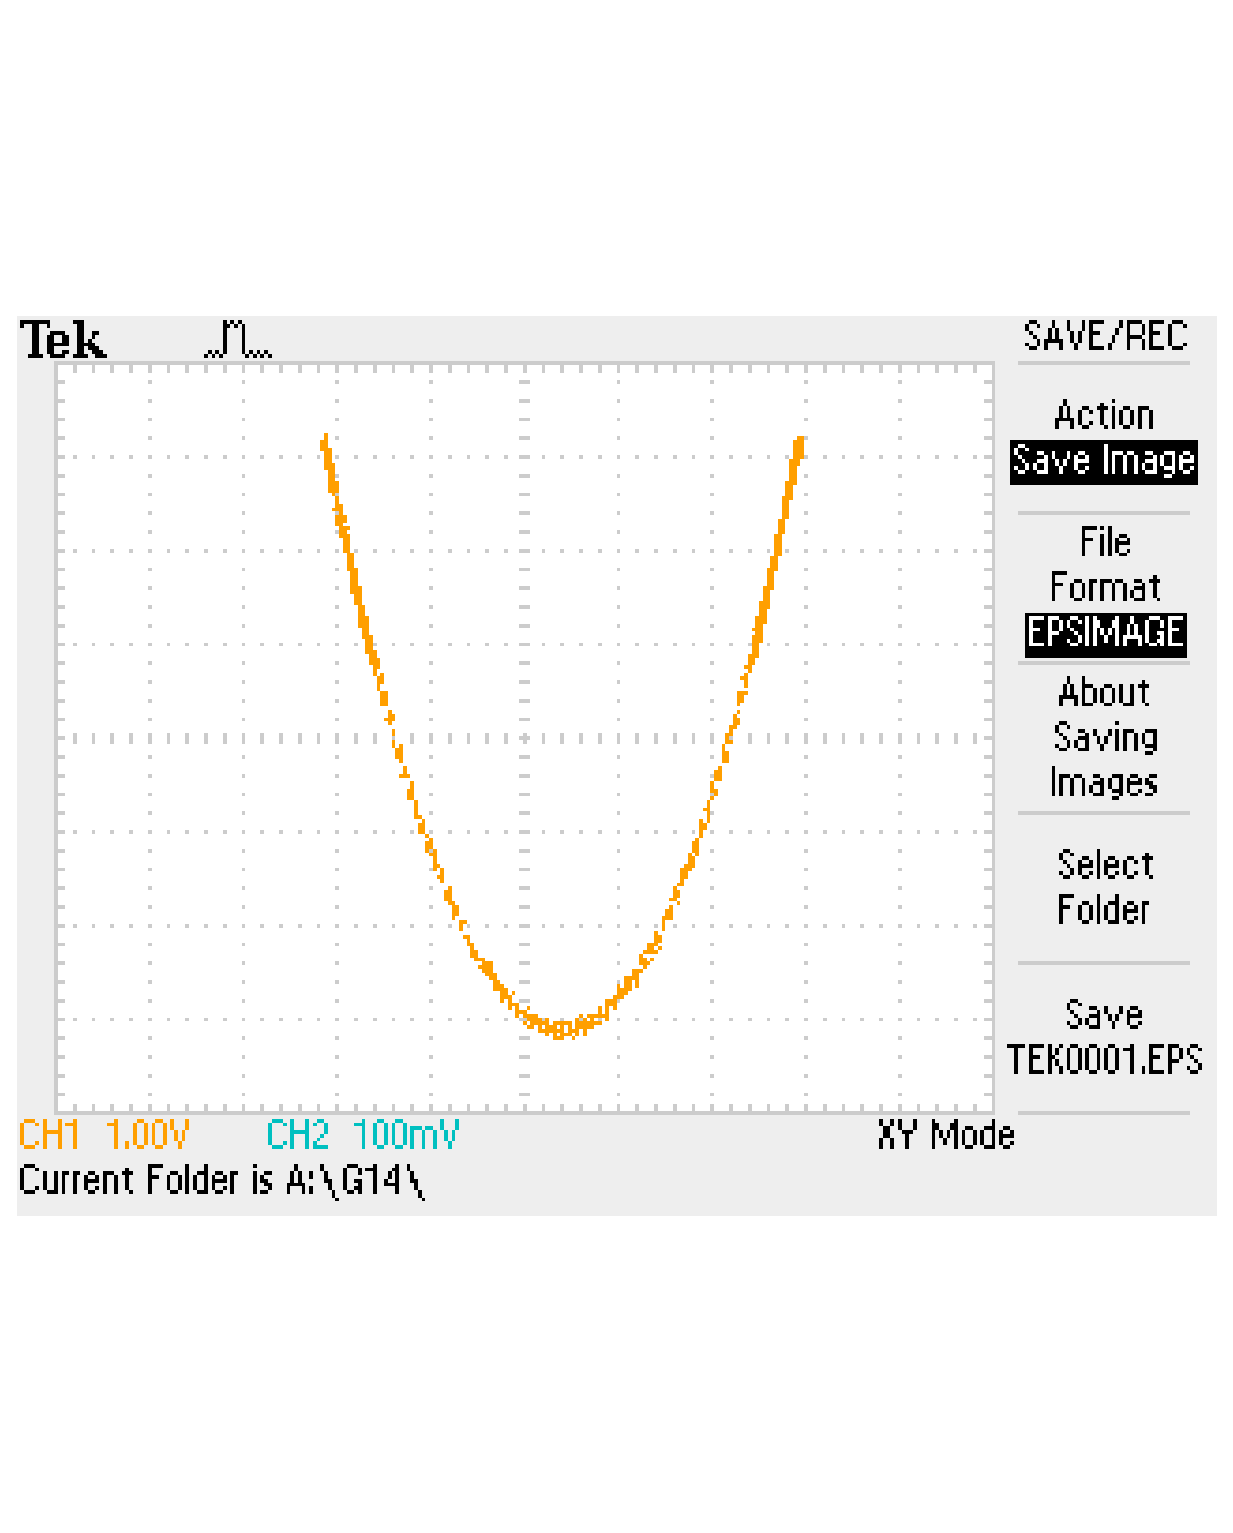
\includegraphics[width=\textwidth,clip,trim={0 5cm 3.4cm 5cm}]{TEK1.eps}
	\end{subfigure}
	\begin{subfigure}{0.49\textwidth}
		\centering
		\includegraphics[width=\textwidth,clip,trim={0 5cm 3.4cm 5cm}]{TEK2.eps}
	\end{subfigure}
	
	\begin{subfigure}{0.49\textwidth}
		\centering
		\includegraphics[width=\textwidth,clip,trim={0 5cm 3.4cm 5cm}]{TEK3.eps}
	\end{subfigure}
	\begin{subfigure}{0.49\textwidth}
		\centering
		\includegraphics[width=\textwidth,clip,trim={0 5cm 3.4cm 5cm}]{TEK4.eps}
	\end{subfigure}
	
	\caption{}
	\label{fig:xy}
\end{figure}


\subsection{Bandpass filter}
\subsubsection{Phase response}

\subsubsection{Gain dependence on frequency}








\section{Johnson's noise \& Boltzmann's constant}

\subsection{Room temperature measurement}

\subsubsection{Dependence on resistance}

\subsubsection{Dependence on Bandwidth}




\subsection{Measurement at $T=77 \, K$}








\section{Conclusion}



\end{document}
